\chapter{Analyse-Klassen-Diagramm}

In diesem Kapitel wird zuerst auf die Klassen, welche für die Implementierung nötig sind, eingegangen bevor die Abhängigkeiten zwischen diesen Klassen nochmal übersichtlich mittel eines Analyse-Klassen-Diagramms dargestellt werden.

\section{Klassen}
\begin{multicols}{2}
\begin{itemize}
    \item Kunde
    \item Adresse
    \item Vertrag
    \item Mitarbeiter
    \item Rolle
    \item Buchung
    \item Fahrzeug
    \item Fahrzeugklasse
    \item Bild
    \item Reifensatz
    \item Reifen
    \item Kennzeichen
    \item Ausrüstung
    \item Rechnung
    \item Mahnung
    \item Standort
    \item Filiale
    \item Rabattaktion
    \item Backup
    \item Hundetransportbox
\end{itemize}
\end{multicols}


\textbf{Kunde}: Die Kunden-Klasse stellt die Kunden dar und beinhaltet Attribute für alle Informationen, welche für die Identifikation und die Ausstellung von Rechnungen notwendig sind. Dazu besitzt die Klasse jeweils Assoziationen zu Adresse und Vertrag. Zusätzlich wird für die Identifikation eine ID gespeichert. Damit die Mitarbeiter mit dem Kunden einfacher in Kontakt treten können wird ebenfalls eine Mail-Adresse und eine Telefonnummer gespeichert. 

\textbf{Adresse}: Die Adresse wird in Straße, Hausnummer, Ort und Postleitzahl aufgeteilt. Mit der Adress-Klasse werden die Adressen der Kunden dargestellt.

\textbf{Vertrag}: Die Vertrags-Klasse bildet die Verträge ab, welche die Kunden bindet. Dazu wird neben dem Vor- und Nachnamen der Pfad gespeichert, unter welchem die Vertrags-Datei (PDF) zu finden ist.

\textbf{Mitarbeiter}: Die Klasse 'Mitarbeiter' stellt die Mitarbeiter des Unternehmens dar. Da die Mitarbeiter unterschiedliche Aufgaben und dementsprechend unterschiedliche Rollen in der Anwendung haben, steht die Mitarbeiter-Klasse in Assoziation zur Klasse 'Rolle'. Um einen Überblick über Anzahl der Mitarbeiter der Verschiedenen Standorte und Filialen zu erhalten gibt es ebenfalls eine Assoziation zur Klasse 'Filiale'. Für die Sicherung dieser und allen anderen Daten des Systems sollen Backups erstellt werden können, welche auf einen Mitarbeiter zurückführbar sein sollen. Daher muss die Mitarbeiter-Klasse auch in Assoziation zur Klasse 'Backup' stehen.

\textbf{Rolle}: Mit den Rollen sollen die Rechte innerhalb der Anwendung verteilt werden können. Dazu stellt die Klasse 'Rolle' neben dem Rollenname für alle Funktionen der Anwendung jeweils ein Attribut bereit, welches vom Datentyp Boolean ist und angibt, ob ein Nutzer mit dieser Rolle Zugriff auf die entsprechende Funktion haben soll. Damit alle Mitarbeiter mit der gleichen Rolle auf einmal abgerufen werden können, steht die Klasse 'Rolle' in Assoziation mit der Mitarbeiter-Klasse.

\textbf{Buchung}:Die Buchung wird als Koordinator-Klasse zwischen dem Kunden und dem Mitarbeiter dargestellt. Diese Klasse stellt einen vereinbarten Termin für die Mietung eines Autos dar. Dazu wird der Mitarbeiter, welcher die Buchung angelegt hat zusammen mit dem Kunden und dem Datum sowie der Uhrzeit des Termins gespeichert. Außerdem steht die Klasse 'Buchung' in Assoziation mit der Fahrzeug-Klasse, um festlegen zu können, welches Auto gemietet werden soll. Da bei einer Buchung eines Fahrzeugs der Preis durch Rabattaktionen beeinflusst werden kann, steht die Buchungs-Klasse in Assoziation mit der Klasse 'Rabattaktion'. Nach dem Termin soll dem Kunden eine Rechnung mit den Buchungsdaten geschickt werden, weshalb es zusätzlich noch eine Assoziation zwischen 'Buchung' und 'Rechnung' geben muss.

\textbf{Fahrzeug}: Die Klasse Fahrzeuge ist für das abbilden der Fahrzeuge zuständig. Jedes Fahrzeug ist dabei einer Fahrzeugklasse zugeordnet.

\textbf{Fahrzeugklasse}: Die Fahrzeugklassen sind für das unterteilen der Fahrzeuge in verschiedene Kategorien zuständig. Diese Kategorien werden mit der Klasse 'Fahrzeugklasse' dargestellt. Eine Kategorie zeichnet sich dabei durch einen Namen, einen Preis und den benötigten Führerschein aus.

\textbf{Bild}:Die Klasse Bild stellt die Bilder der Fahrzeuge dar. Jedes Bild ist einem Fahrzeug zugeordnet, weshalb die Klasse 'Bild' in Assoziation mit der Klasse 'Fahrzeug' steht. Als weitere Attribute besitzt diese Klasse den Titel des Bildes sowie den Pfad, an welchem das Bild liegt.

\textbf{Reifensatz}: Ein Reifensatz ist einem Fahrzeug zugeordnet, weshalb zwischen diesen beiden Klassen eine Assoziation besteht. Jeder Reifensatz besteht zudem aus vier Reifen und potentiell einem weiteren Reifen (Ersatzreifen).

\textbf{Reifen}: Die Klasse Reifen stellt die Reifen der Fahrzeuge dar. Ein Reifen wird hierbei durch den Hersteller, das Modell, den Zeitpunkt der Herstellung, die Profiltiefe und die Fahrtrichtung beschrieben.

\textbf{Kennzeichen}: Das Kennzeichen dient der Identifikation eines Fahrzeugs. Um das Kennzeichen eines Fahrzeugs in der Anwendung darzustellen wird die Klasse 'Kennzeichen' implementiert, welche die Zulassungsstelle, die Art des Kennzeichens und eine Zeichenkette für das eigentliche Kennzeichen als Attribute enthält.

\textbf{Ausrüstung}: Die Klasse 'Ausrüstung' stellt die Ausrüstung eines Fahrzeugs dar. Dabei handelt es sich nicht um die Ausstattung des Fahrzeugs (Klimaanlage, Panoramaschiebedach, ...) sondern um Fahrradträger, Dachbox und Hundetransportbox. Die Klasse 'Ausrüstung' ist fungiert dabei als Oberklasse der Ausrüstungsgegenstände und besitzt als Attribute die Kompatibilität mit den verschiedenen Fahrzeugen und das Fahrzeug, welches den Gegenstand momentan ausgerüstet hat.

\textbf{Rechnung}: Eine Rechnung fällt immer nach dem Abschluss einer Fahrt an. Die Klasse 'Rechnung' bildet solch eine Rechnung ab und beinhaltet Methoden um basierend auf der Buchung eine Rechnung zu erstellen und an den Kunden zu versenden.

\textbf{Mahnung}: Wenn der Kunde die Rechnung nicht im vorgegebenen Zeitraum begleicht, wird eine Mahnung versendet. Die Klasse 'Mahnung' bildet solch eine Rechnung ab und beinhaltet Methoden, um basierend auf der Rechnung eine Mahnung zu erstellen und um diese anschließend an den Kunden zu versenden.

\textbf{Standort}: Das Unternehmen ist an verschiedensten Standorten tätig. Um diese Standorte abzubilden wird eine Klasse 'Standort' implementiert, welche in Assoziation mit den Klassen 'Fahrzeug' und 'Filiale' steht. Dadurch können dem Standort alle Mitarbeiter und Fahrzeuge zugeordnet werden.
Des Weiteren wird der Standort durch eine Beschreibung und einen Namen beschrieben.

\textbf{Filiale}: Die Klasse 'Filiale' stellt eine Filiale des Unternehmens dar. Dafür wird die Filiale sowohl mit dem Standort als auch mit den Mitarbeitern sowie einer Adresse in Assoziation gesetzt. Außerdem besitzt diese Klasse die Anzahl der Mitarbeiter als Attribut.  

\textbf{Rabattaktion}:Mit der Klasse 'Rabattaktion' werden die Rabattaktionen dargestellt. Dazu besitzt diese Klasse den prozentualen Preisnachlass und den Namen der Rabattaktion als Attribute.

\textbf{Backup}: Die Klasse Backup ist für die Darstellung der Backups zuständig. Dafür wird zum einen das Datum und die Uhrzeit der Erstellung des Backups und zum anderen der Pfad, unter welchem das Backup abgelegt wurde, als Attribut bereitgestellt.

\textbf{Hundetransportbox}: Die Hundetransportbox ist eine der Unterklassen der Ausrüstung, welche die Klasse 'Ausrüstung' um folgende Attribute erweitert: Das Maximalgewicht des Hundes, Höhe, Breite und Länge sowie das Volumen.

\textbf{Fahrradträger}: Ein Fahrradträger ist ebenfalls ein Teil der Ausrüstung und somit eine Unterklasse der Klasse 'Ausrüstung'. Die Klasse Fahrradträger hat zusätzlich Attribute für die Anzahl der Fahrräder, welche mit dem Fahrradträger Transportiert werden können, und das Maximale Gewicht, mit welchem der Fahrradträger beladen werden darf.

\textbf{Dachbox}: Die letzte Unterklasse der Ausrüstung ist die Dachbox, welche zusätzlich Attribute für das Volumen und die Abschließbarkeit der Dachbox besitzt.


\newpage


\section{Diagramm}

\begin{figure}[!ht]
    \centering
    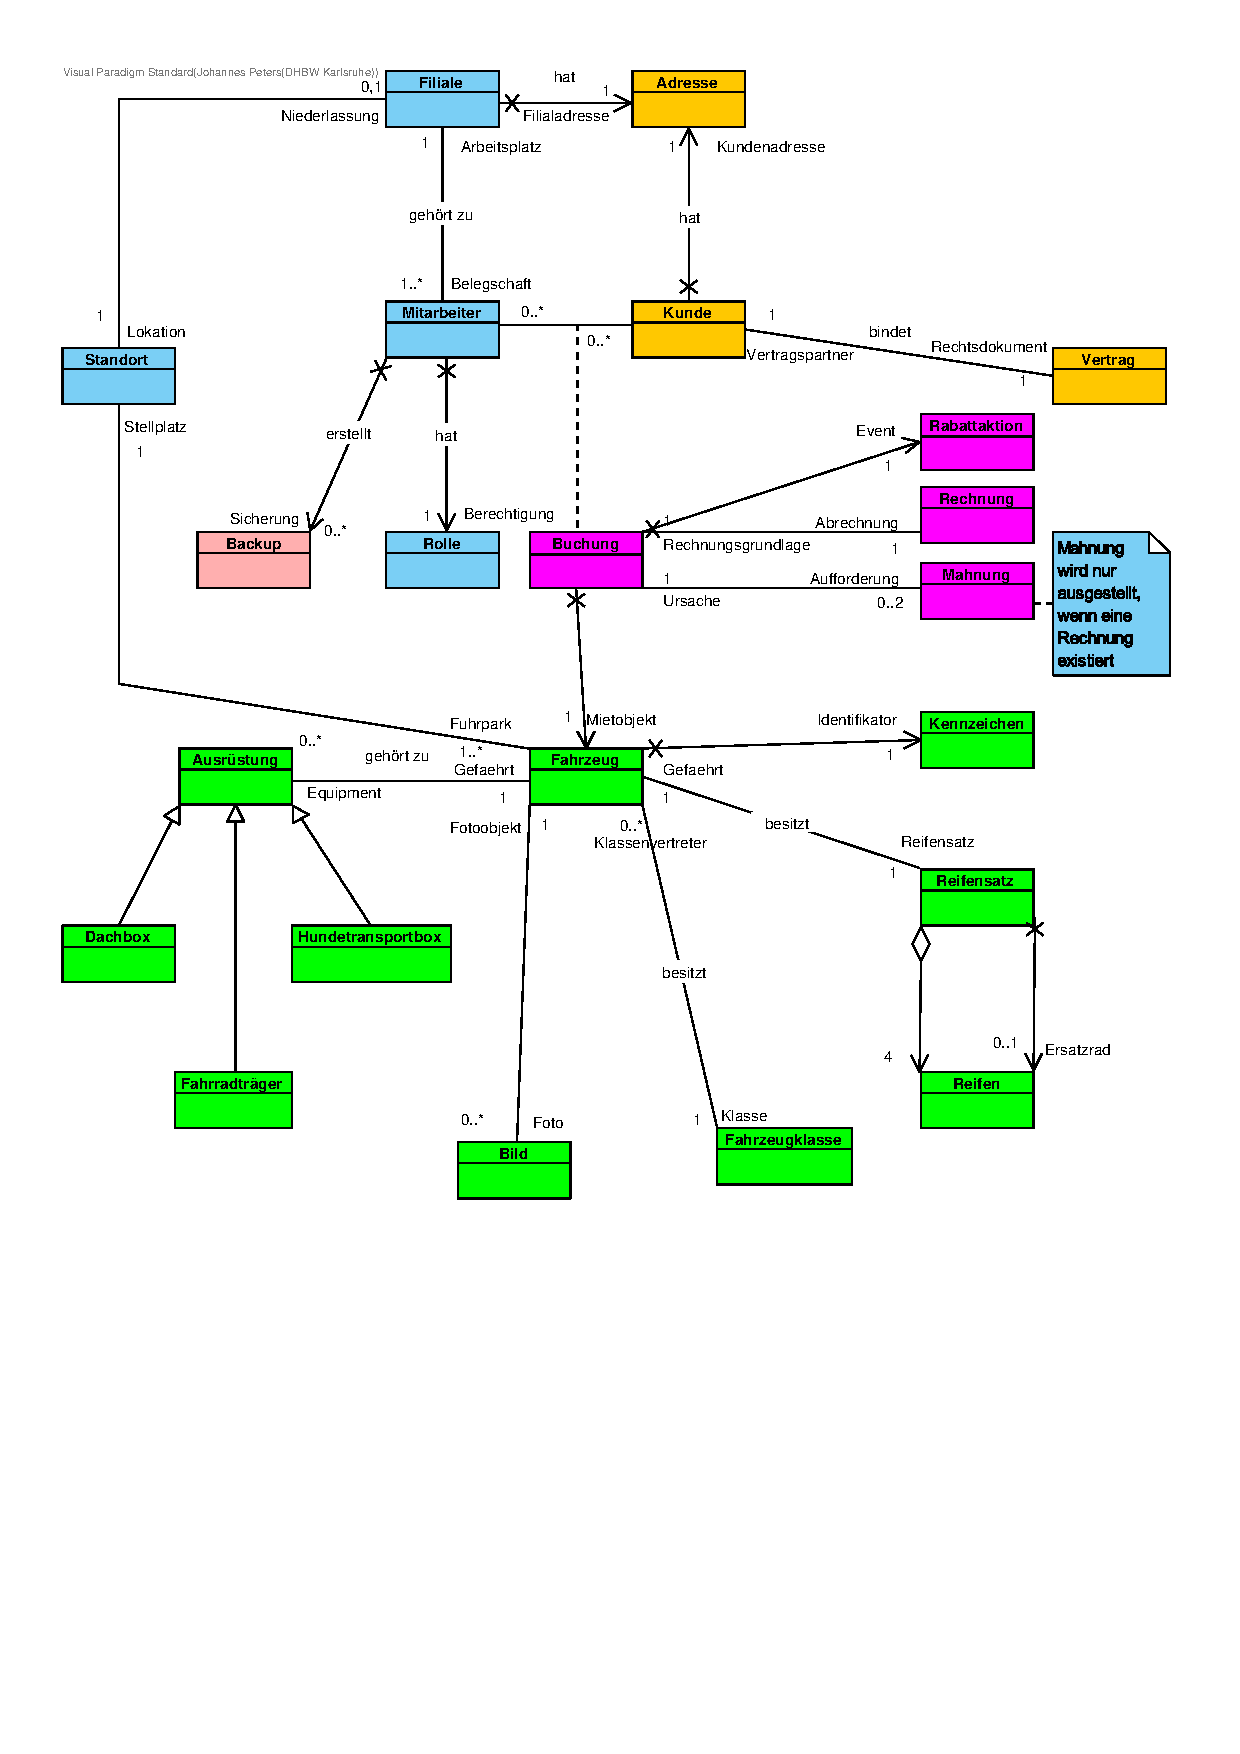
\includegraphics[width=\textwidth, trim = 0cm 10cm 0cm 0cm]{Bilder/Diagramme/Analyseklassendiagramm.pdf}
    \caption{Analyseklassendiagramm}
    \label{img:akd}
\end{figure}